\documentclass[12pt, a4paper, oneside]{ctexart}
\usepackage{amsmath, amsthm, amssymb, bm, color, framed, graphicx, hyperref, mathrsfs}
\usepackage{tikz}

\title{\textbf{3月16日作业}}
\author{韩岳成 524531910029}
\date{\today}
\linespread{1.5}
\definecolor{shadecolor}{RGB}{241, 241, 255}
\newcounter{problemname}
\newenvironment{problem}{\begin{shaded}\stepcounter{problemname}\par\noindent\textbf{题目\arabic{problemname}. }}{\end{shaded}\par}
\newenvironment{solution}{\par\noindent\textbf{解答. }}{\par}
\newenvironment{note}{\par\noindent\textbf{题目\arabic{problemname}的注记. }}{\par}
\everymath{\displaystyle}

\begin{document}

\maketitle

\begin{problem}
    证明：若$G$是连通简单图但不是完全图，则$G$中必存在三个顶点$u,v$和$w$，使得$uv, vw \in E(G)$ 而 $uw \notin E(G)$.
\end{problem}

\begin{solution}
    根据完全图的定义，若图$G$不为完全图，则至少存在一对顶点在图$G$中不相邻，记这对顶点为$u, 2$，满足$uw \notin E(G)$.

    由于$G$为连通简单图，则存在一条从$u$到$w$的路径：
    \[ P : u=v_0,v_1,v_2,\cdots,v_k=w\]

    我们考虑$v_0, v_1, v_2$，已知$v_0v_1\in E(G), v_1v_2 \in E(G)$.
    \begin{itemize}
        \item 若$v_0v_2 \notin E(G)$，则$v_0, v_1, v_2$这三个点满足命题。
        \item 若$v_0v_2 \in E(G)$，则我们可以将路径缩短为$P' : v_0, v_2,\cdots, v_k$，继续对$v_0, v_2, v_3$进行讨论。
    \end{itemize}
    如此递归下去，如果对每一个$v_0, v_i (i \le k-1)$ 都有 $v_0v_i \in E(G)$，我们可以不断缩短路径，直到路径上只剩下$v_0, v_{k-1}, v_k$三个点。已知$v_0v_k \notin E(G)$，则$v_0, v_{k-1}, v_k$满足题设条件。否则若存在$v_i$使得对于所有$0<j<i$都有$v_0v_j \in E(G)$，但$v_0v_i \notin E(G)$，则$v_0, v_{i-1}, v_i$满足题设条件。命题得证。
\end{solution}

\begin{problem}
(1) 举反例说明如下命题不成立：如果$e$是图$G$的一条割边，则$e$至少有一个端点是$G$的割点.

(2) 试添加一个假设条件使其成立，并证明所得命题的正确性.
\end{problem}

\begin{solution}
    (1)
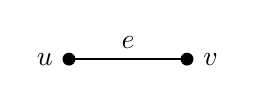
\begin{tikzpicture}
    % 定义节点
    \node[circle, draw, fill=black, inner sep=1.5pt, label=left:$u$] (u) at (0,0) {};
    \node[circle, draw, fill=black, inner sep=1.5pt, label=right:$v$] (v) at (1.5,0) {};
    
    % 连接边
    \draw[thick] (u) -- (v) node[midway, above] {$e$};
\end{tikzpicture}

    (2) 添加条件：设 $e = (u, v)$ 是图 $G$ 的一条割边，且 $\max(d(u), d(v)) \ge 2$。

    证明：由于 $e=(u, v)$ 是割边，根据定义，删除边 $e$ 后，图 $G$ 的连通分支数增加。这意味着在原图 $G$ 中，任意一条连接 $u$ 和 $v$ 的路径都必须经过边 $e$。

    反证假设 $u$ 和 $v$ 都不是割点。不妨假设$d(u)\ge 2$.
    根据割点的定义，若 $u$ 不是割点，则 $G-u$ 是连通的；

    由于 $d(u) \ge 2$，在原图中，$u$ 除了连接 $v$ 的边 $e$ 之外，至少还连接着另一个顶点 $w$（即 $uw \in E(G), w \neq v$）。

    考虑图 $G-e$。在 $G-e$ 中，$u$ 和 $v$ 分别属于两个不同的连通分支 $G_u$ 和 $G_v$（因为 $e$ 是割边）。

    现在考虑删除顶点 $u$ 后的图 $G-u$。因为 $d(u) \ge 2$，删去 $u$ 后，$u$ 的邻居 $w$ 依然保留在图中。
    若 $u$ 不是割点，意味着在 $G-u$ 中，原先与 $u$ 相邻的所有点（包括 $v$）依然在同一个连通分支中。
    这意味着在 $G-u$ 中，存在一条从 $w$ 到 $v$ 的路径。将边 $(w, u)$ 补回，便得到了一条不经过 $e=(u,v)$ 的从 $u$ 到 $v$ 的路径。
    这与$e$ 是割边相矛盾。

    因此假设不成立，故 $u$ 或 $v$ 中至少有一个必须是$G$的割点。
\end{solution}

\begin{problem}
证明：点$v$是图$G$的割点当且仅当$v$至少属于$G$的两个不同的块.
\end{problem}

\begin{solution}
    设 $G$ 是一个连通图。根据块的定义，块是图的极大连通子图且不含割点。

\textbf{充分性：}
假设 $v$ 同时属于两个不同的块 $B_1$ 和 $B_2$。

因为 $B_1 \neq B_2$，且块的性质规定任意两个不同的块至多共用一个顶点，因此 $B_1 \cap B_2 = \{v\}$。既然 $B_1 \neq B_2$，则存在顶点 $u \in V(B_1) \setminus \{v\}$ 和 $w \in V(B_2) \setminus \{v\}$。

在图 $G$ 中，从 $u$ 到 $w$ 的路径必须经过 $v$。因为如果存在一条不经过 $v$ 的路径 $P$ 连接 $u$ 和 $w$，则 $P \cup B_1 \cup B_2$ 将构成一个更大的连通子图。且该连通子图内部不再含有割点（因为 $v$ 不再是该更大子图的割点），这与 $B_1$ 和 $B_2$ 是“极大”连通子图的定义相矛盾。

因此，$G-v$ 不再连通，故 $v$ 是 $G$ 的割点。


\textbf{必要性：}
假设 $v$ 是 $G$ 的割点。

根据割点的定义，删除 $v$ 后的图 $G-v$ 至少存在两个连通分支，设每个连通分支为 $C_1, C_2, \dots, C_k$ ($k \ge 2$)。

考虑 $C_i \cup \{v\}$ 诱导出的子图 $G_i$。由于 $G$ 是连通的，$v$ 必须与每个分支 $C_i$ 中的至少一个顶点相邻。
每个 $G_i$ 包含至少一个块 $B_i$，且 $v \in V(B_i)$。

若 $B_1 = B_2$，则意味着 $C_1$ 中的顶点和 $C_2$ 中的顶点在不经过 $v$ 的情况下存在于同一个块中，这与 $C_1$ 和 $C_2$ 是 $G-v$ 中不同的连通分支（即在 $G-v$ 中它们互不连通）相矛盾。

因此，$B_1$ 和 $B_2$ 必定是不同的块。从而，$v$ 至少属于 $B_1$ 和 $B_2$ 这两个不同的块。


综上所述，命题得证。
\end{solution}
\end{document}